\documentclass[
  12pt,
  openright,
  twoside,
  a4paper,
  english,
  french,
  spanish,
  brazil
]{abntex2}

%
% Pacotes
%
\usepackage{lmodern}
\usepackage[T1]{fontenc}
\usepackage[utf8]{inputenc}
\usepackage{indentfirst}
\usepackage{color}
\usepackage{graphicx}
\usepackage{microtype}
\usepackage{pdfpages}
\usepackage{xltabular}
\usepackage{customizations}

%
% Pacotes de citações
%
\usepackage[brazilian,hyperpageref]{backref}
\usepackage{abntex2cite}

%
% Configurações de pacotes
%
\renewcommand{\backrefpagesname}{Citado na(s) página(s):~}
\renewcommand{\backref}{}
\renewcommand*{\backrefalt}[4]{
	\ifcase #1
		Nenhuma citação no texto.
	\or
		Citado na página #2.
	\else
		Citado #1 vezes nas páginas #2.%
	\fi
}

%
% Informações de dados para a capa e folha de rosto
%
\titulo{Projeto Integrador de Engenharia 1}
\autor{Grupo 01 (T01)}
\local{Brasília, DF}
\data{2024, v1.1.0}
\instituicao{Universidade de Brasília \par Faculdade do Gama}
\tipotrabalho{Relatório técnico}
\preambulo{
  Trabalho submetido à disciplina de Projeto Integrador de Engenharia 1 da
  Universidade de Brasília, ministrada pelo professor Diogo Garcia.
}
\orientador{Diogo Garcia}

% Informações do PDF
\makeatletter
\hypersetup{
  pdftitle={\@title},
  pdfauthor={\@author},
  pdfsubject={\imprimirpreambulo},
  pdfcreator={LaTeX with abnTeX2},
  pdfkeywords={abnt}{latex}{abntex}{projeto integrador de engenharia 1},
  colorlinks=true,
  linkcolor=blue,
  citecolor=blue,
  filecolor=magenta,
  urlcolor=blue,
  bookmarksdepth=4
}
\makeatother

%
% Configurações de aparência do PDF final
%
\definecolor{blue}{RGB}{41,5,195} % Cor azul para os links

% Posiciona figuras e tabelas no topo da página quando adicionadas sozinhas
% em um página em branco. Ver https://github.com/abntex/abntex2/issues/170
\makeatletter
\setlength{\@fptop}{5pt}
\makeatother

% Possibilita criação de Quadros e Lista de quadros.
% Ver https://github.com/abntex/abntex2/issues/176
\newcommand{\quadroname}{Quadro}
\newcommand{\listofquadrosname}{Lista de quadros}

\newfloat[chapter]{quadro}{loq}{\quadroname}
\newlistof{listofquadros}{loq}{\listofquadrosname}
\newlistentry{quadro}{loq}{0}

% configurações para atender às regras da ABNT
\setfloatadjustment{quadro}{\centering}
\counterwithout{quadro}{chapter}
\renewcommand{\cftquadroname}{\quadroname\space}
\renewcommand*{\cftquadroaftersnum}{\hfill--\hfill}

% Ver https://github.com/abntex/abntex2/issues/176
\setfloatlocations{quadro}{hbtp}

%
% Espaçamentos entre linhas e parágrafos
%
\setlength{\parindent}{1.3cm}
\setlength{\parskip}{0.2cm}

%
% Início do documento
%
\begin{document}

\selectlanguage{brazil}
\frenchspacing

%
% Elementos pré-textuais
%
\pretextual

%
% Capa
%
\imprimircapa

%
% Folha de rosto
% (o * indica que haverá a ficha bibliográfica)
%
\imprimirfolhaderosto*

\begin{fichacatalografica}
	\sffamily
	\vspace*{\fill}
	\begin{center}
    \fbox{
      \begin{minipage}[c][8cm]{13.5cm}
        \small
        \imprimirautor
        %Sobrenome, Nome do autor

        \hspace{0.5cm} \imprimirtitulo  / \imprimirautor. --
        \imprimirlocal, \imprimirdata-

        \hspace{0.5cm} \thelastpage p. : il. (algumas color.) ; 30 cm.\\

        \hspace{0.5cm} \imprimirorientadorRotulo~\imprimirorientador\\

        \hspace{0.5cm}
        \parbox[t]{\textwidth}{\imprimirtipotrabalho~--~\imprimirinstituicao,
        \imprimirdata.}\\

        \hspace{0.5cm}
          1. Projeto Integrador de Engenharia 1.
          2. Faculdade UnB Gama.
          I. Professor Diogo Garcia.
          II. Universidade de Brasília.
      \end{minipage}
    }
	\end{center}
\end{fichacatalografica}

%
% Inserir folha de aprovação
%

% Isto é um exemplo de Folha de aprovação, elemento obrigatório da NBR
% 14724/2011 (seção 4.2.1.3). Você pode utilizar este modelo até a aprovação
% do trabalho. Após isso, substitua todo o conteúdo deste arquivo por uma
% imagem da página assinada pela banca com o comando abaixo:
%
% \begin{folhadeaprovacao}
%   \includepdf{folhadeaprovacao_final.pdf}
% \end{folhadeaprovacao}
%
\begin{folhadeaprovacao}
  \begin{center}
    {\ABNTEXchapterfont\large\imprimirautor}

    \vspace*{\fill}\vspace*{\fill}
    \begin{center}
      \ABNTEXchapterfont\bfseries\Large\imprimirtitulo
    \end{center}
    \vspace*{\fill}

    \hspace{.45\textwidth}
    \begin{minipage}{.5\textwidth}
        \imprimirpreambulo
    \end{minipage}%
    \vspace*{\fill}
   \end{center}

   Trabalho aprovado. \imprimirlocal, 24 de abril de 2024:

   \assinatura{\textbf{\imprimirorientador} \\ Orientador}
   \assinatura{\textbf{Rafael Rodrigues} \\ Coorientador}
   \assinatura{\textbf{Jungpyo Lee} \\ Coorientador}
   \assinatura{\textbf{Juliana Petrocchi} \\ Coorientador}
   \assinatura{\textbf{Ricardo Ajax} \\ Coorientador}

   \begin{center}
    \vspace*{0.5cm}
    {\large\imprimirlocal}
    \par
    {\large\imprimirdata}
    \vspace*{1cm}
  \end{center}
\end{folhadeaprovacao}

%
% Dedicatória
%
\begin{dedicatoria}
  \vspace*{\fill}
  \centering
  \noindent
  \textit{
    Dedicamos este trabalho aos nossos orientadores, que durante o semestre nos
    proporcionaram a melhor experiência para escrever um trabalho de qualidade.
  }
  \vspace*{\fill}
\end{dedicatoria}

%
% TODO: Agradecimentos
%

%
% Resumo
%
% Ajusta o espaçamento dos parágrafos do resumo
\setlength{\absparsep}{18pt}
\begin{resumo}
  O seguidor de linha, também chamado de \textit{follow line} ou
  \textit{line follower robot}, é uma categoria de robôs autônomos geralmente
  semelhantes a carros de corrida cujo objetivo é realizar um percurso no menor
  tempo possível seguindo uma linha preta no chão. Este trabalho apresenta o
  projeto de um seguidor de linha que utiliza circuitos eletrônicos, sensores e
  softwares para realizar três percursos aleatórios. Além de percorrer os
  trajetos, o robô também deve ser capaz de carregar um ovo sem quebrá-lo, e
  apresentar dados de telemetria em algum dispositivo externo. O projeto
  foi desenvolvido por estudantes de engenharia da Universidade de Brasília
  durante a disciplina de Projeto Integrador de Engenharia 1, ministrada pelo
  professor Diogo Garcia.

  \textbf{Palavras-chave}:
    Seguidor de linha. Carrinho seguidor de linha. Engenharia. Projeto
    Integrador de Engenharia 1. Universidade de Brasília. Faculdade do Gama.
    Diogo Garcia.
\end{resumo}


%
% Inserir lista de ilustrações
%
\pdfbookmark[0]{\listfigurename}{lof}
\listoffigures*
\cleardoublepage

%
% Inserir lista de quadros
%
\pdfbookmark[0]{\listofquadrosname}{loq}
\listofquadros*
\cleardoublepage

%
% Inserir lista de tabelas
%
\pdfbookmark[0]{\listtablename}{lot}
\listoftables*
\cleardoublepage

%
% inserir lista de abreviaturas e siglas
%
\begin{siglas}
  \item[FGA] Faculdade do Gama
  \item[INATEL] Instituto Nacional de Telecomunicações
  \item[ANATEL] Agência Nacional de Telecomunicações
  \item[IFR] \textit{International Federation of Robotics}
  \item[PLA] \textit{Polylactic Acid}
  \item[MDF] \textit{Medium-density Fibreboard}
\end{siglas}

%
% Inserir lista de símbolos
%
\begin{simbolos}
  \item[$ \Lambda $] Lambda (maiúsculo)
\end{simbolos}

%
% Inserir sumário
%
\pdfbookmark[0]{\contentsname}{toc}
\tableofcontents*
\cleardoublepage

\textual

\chapter{Introdução}

Um seguidor de linha é um robô autônomo que segue uma linha preta no chão. O
objetivo é percorrer um percurso no menor tempo possível, evitando obstáculos e
mantendo-se dentro dos limites da pista. De acordo com a INATEL, a definição de
um seguidor de linha é:

\begin{citacao}
  \lbrack...\rbrack 
  \space
  uma categoria de robôs autônomos que, na maioria das vezes, se assemelham a
  carros de corrida. Através da combinação de motores, sensores e inteligência
  artificial, o principal objetivo é percorrer um determinado percurso no menor
  tempo possível. Os métodos utilizados, como mapeamento e a diferenciação entre
  retas e curvas, para que a estrutura mecânica tenha o melhor aproveitamento,
  podem ser empregados em diversos métodos de controle.
  \cite{INATEL:Seguidor-de-Linha}
\end{citacao}

Essa definição destaca a importância da integração de diferentes conceitos e
tecnologias para o desenvolvimento de um seguidor de linha eficiente. A
combinação de motores, sensores e algoritmos de controle é essencial para
garantir que o robô possa navegar com precisão e rapidez, evitando colisões e
desvios da linha de referência. Além disso, a capacidade de diferenciar entre
retas e curvas e de realizar mapeamentos do ambiente são aspectos fundamentais
para o desempenho do robô em diferentes cenários.

Uma vez que os robôs têm, frequentemente, um propósito de competição, a diretriz
que o projeto deve seguir varia da competição ou propósito final. No Brasil, não
existem quaisquer proibições sobre pequenos robôs seguidores de linha, as
possíveis legislações que podem abranger esse robô variam de acordo com seu
propósito, como se ele irá ou não ser comercializado \cite{Lei:8078:1990}, se
ele utiliza ou não formas sem fio para sua partida, de acordo com as
conformidades da ANATEL \cite{ANATEL:Manual-de-Orientacoes}, e se possuindo uma
câmera, ela faz registro e armazenamento das gravações \cite{Lei:12651:2012}.
Por fim, é responsabilidade dos construtores do robô não infringir leis como a
Lei de Propriedade Intelectual \cite{Lei:9279:1996} e respeitar a privacidade e
os direitos pessoais.

A indústria de robótica tem experimentado um crescimento significativo nos
últimos anos, impulsionado pelo avanço das tecnologias de automação e pela
demanda crescente por soluções inteligentes em diversos setores. Dentro desse
cenário, os seguidores de linha se destacam como uma aplicação prática e
educativa da robótica, especialmente popular entre entusiastas de tecnologia e
em ambientes educacionais. No entanto, o mercado atual para carrinhos
seguidor de linha é caracterizado por um alto custo de produtos similares, que
muitas vezes limita a acessibilidade para uma base mais ampla de consumidores.
Além disso, o número reduzido de empresas concorrentes pode restringir a
variedade e inovação de produtos disponíveis.

% Pular para a próxima página. Segundo as normas da ABNT,
% parágrafos não devem ser divididos entre páginas.
\clearpage

% TODO: Colocar referência correta do artigo citado abaixo.
Segundo Makedon, Mykhailenko e Vazov:

\begin{citacao}
  \lbrack...\rbrack 
  \space
  o nível de automação na indústria automotiva é geralmente muito mais alto do
  que em todos os outros setores. Desde 2014, um número significativo de robôs
  industriais foi entregue às empresas da indústria automobilística sul-coreana.
  \lbrack...\rbrack\space De acordo com especialistas da IFR, projetos para a
  produção de baterias para carros híbridos e veículos elétricos podem ser a
  fonte de um aumento significativo na densidade de robotização.
  \cite[p.~6]{Makedon:Dominants-and-Features-Market-Robotics}

\end{citacao}

Essas tendências globais destacam a importância da automação em vários setores,
inclusive na indústria de seguidores de linha, que pode se beneficiar da
integração de novas tecnologias para aprimorar a eficiência e a acessibilidade.

Neste trabalho, propomos o desenvolvimento de um carrinho seguidor de linha
autônomo, que seja capaz de percorrer trajetos pré-definidos sem auxílio
externo, além de transportar um ovo sem quebrá-lo, e enviar dados de telemetria,
como o trajeto percorrido, a velocidade instantânea, a aceleração instantânea, o
consumo energético e o tempo de percurso, para um dispositivo externo ao robô.

\chapter{Termo de Abertura do Projeto}

\section{Dados do Projeto}

\begin{center}
  \begin{tabular}{|l|l|}
    \hline
    \textbf{Nome do Projeto} & Carrinho seguidor de linha \\
    \hline
    \textbf{Data de Abertura} & 17/04/2024 \\
    \hline
    \textbf{Código} & 1-A \\
    \hline
    \textbf{Patrocinador} & Universidade de Brasília \\
    \hline
    \textbf{Gerente} & Sarah Loriato Nazareth Franco (190020008) \\
    \hline
  \end{tabular}
\end{center}

\section{Objetivos}

Os objetivos do projeto são desenvolver um carrinho seguidor de linha autônomo
que seja capaz de percorrer trajetos pré-definidos sem auxílio externo, além de
transportar um ovo sem quebrá-lo. É possível descrever os objetivos do projeto
utilizando o acrônimo \textit{SMART} \cite{SMART-Goals:2017}, que seriam os
seguintes:

\subsection{\textit{Specific} (específico)}

Desenvolver um carrinho que seja capaz de percorrer completamente três
trilhas marcadas no chão, sem auxílio externo para a sua movimentação e
início de trajeto, exceto para ser iniciado.
 
\subsection{\textit{Measurable} (mensurável)}

O sucesso do carrinho será medido através de sua habilidade de completar os
trajetos no menor tempo possível, sem causar dano ao ovo transportado. O
registro de dados como trajetória percorrida, velocidade instantânea,
aceleração instantânea, tempo de percurso e consumo energético ajudará a
mensurar a performance.

\subsection{\textit{Agreed} (acordado)}

O projeto será acordado com as partes interessadas dentro da universidade,
incluindo professores e alunos das diferentes engenharias da FGA, garantindo
uma abordagem multidisciplinar no desenvolvimento do carrinho.

\subsection{\textit{Realistic} (realista)}

O projeto será baseado na realidade do que pode ser alcançado pelos estudantes,
utilizando conhecimentos de todas as engenharias da FGA, respeitando as
restrições impostas pelos professores e pela universidade.

\subsection{\textit{Time-bound} (limitado ao tempo)}

O projeto terá um prazo determinado para sua finalização, alinhado com o
calendário acadêmico e as datas estipuladas para os pontos de controle e
apresentação final.

\section{Mercado-alvo}

O carrinho seguidor de linha é um projeto que visa atender a demanda de
estudantes de engenharia que desejam desenvolver habilidades práticas e
multidisciplinares. Apesar disso, o projeto também pode ser utilizado por
empresas de logística e transporte, particularmente empresas de comércio
atacadista e armazéns no DF e região. Empresas de fazendas verticais, empresas
que visam produzir alimentos de forma eficiente e automatizada em grandes
centros urbanos também podem se beneficiar do projeto.

\chapter{Equipe de Trabalho}

\begin{quadro}[htb]
  \caption{\label{quadro_equipe_trabalho}Equipe de Trabalho}

  \begin{tabular}{|c|c|c|}
    \hline
    \textbf{Nome} & \textbf{Matrícula} & \textbf{Atribuição} \\
    \hline
    Sarah Loriato N. Franco & 190020008 & Gerente geral \\
    \hline
    Guilherme Elizeu de O. Freitas & 150128258 & Gerente de estruturas \\
    \hline
    Pedro Ambrosio A. Bianco & 231029805 & Gerente de qualidade e energia \\
    \hline
    Henrique Galdino Couto & 200058258 & Gerente de software \\
    \hline
    Rafael Silva Frota & 180067460 & Gerente de hardware \\
    \hline
    João Ricardo F. de Almeida & 190046562 & Colaborador de software \\
    \hline
    João Pedro Costa & 190030801 & Colaborador de software \\
    \hline
    Alexandre de Santana Beck & 211061350 & Colaborador de software \\
    \hline
    Rodrigo Braz F. Gontijo & 190116498 & Colaborador de software \\
    \hline
    Luis Felipe de S. Braga & 202016865 & Colaborador de software \\
    \hline
    Caio Alexandre O. Silva & 221007644 & Colaborador de software \\
    \hline
    Thales Germano V. Lima & 202017147 & Colaborador de software \\
    \hline
    Vitor Carvalho Pereira & 211062615 & Colaborador de software \\
    \hline
    Ana Caroline S. Batista & 202063186 & Colaboradora de estruturas \\
    \hline
    Maria Eliza Braga & 221022373 & Colaboradora de estruturas \\
    \hline
  \end{tabular}

  \fonte{Elaborado pelos autores.}
\end{quadro}

\chapter{Projeto Conceitual do Produto}

\section{Características Gerais}

O projeto foi divido em quatro frentes de trabalho, sendo elas:
\textbf{estrutura}, \textbf{hardware}, \textbf{software} e \textbf{energia},
com o intuito de organizar estruturar de forma que os objetivos sejam alcançados
de forma eficiente, seguindo os requisitos estabelecidos pela equipe e pelos
orientadores. As atribuições das quatro frentes serão realizadas em paralelo, de
modo a garantir que a integração e o funcionamento das mesmas esteja de acordo
com o esperado inicialmente.

\subsection{Estrutura}

Será responsável pela definição, aquisição e montagem dos materiais necessários
para elaboração da estrutura do carrinho. Para alcançar os objetivos previstos,
a estrutura apresentada deverá sustentar e proteger um ovo de galinha durante a
execução dos trajetos determinados.

\subsection{Hardware}

Será responsável pela definição, aquisição e configuração dos componentes
eletrônicos que serão utilizados na elaboração do carrinho, além de garantir a
medição de dados em tempo real para trajetória percorrida, velocidade
instantânea, aceleração instantânea, tempo de percurso e consumo energético.

\subsection{Software}

Será responsável pela definição, documentação e programação dos códigos que
serão utilizados para definir o funcionamento do carrinho, além de realizar os
cálculos e armazenamento dos dados de trajetória percorrida, velocidade
instantânea, aceleração instantânea, tempo de percurso e consumo energético, e
enviar esses dados para um dispositivo externo para visualização.

\subsection{Energia}

Será responsável pela definição, aquisição e montagem dos componentes que
alimentarão o carrinho e seus demais componentes, além de efetuar o cálculo e
medições dos relacionados ao consumo energético do mesmo.

\section{Estrutura Analítica}

Para o desenvolvimento do projeto, diversos fatores devem ser levados em
consideração de forma a facilitar a integração entre as frentes e a orientação
do projeto como um todo. A coleta e a análise dos dados coletados deverão ser
feitas de maneira precisa e coerente, utilizando técnicas e ferramentas que
permitam persistir e agrupar os valores obtidos em variáveis de banco de dados,
de forma a atender requisitos previamente estabelecidos para distância e tempo.

As atividades realizadas pelas frentes serão integradas e, por isto, deverão ser
executadas com rigor e exigem uma comunicação constante e eficaz entre as
partes, visando garantir uma melhor desenvolvimento do produto. As frentes de
software e hardware deverão trabalhar juntas no que diz respeito a integração
dos circuitos e componentes eletrônicos com os códigos e programas responsáveis
pelos movimentos e cálculos necessários para o projeto.

A frente de consumo energético trabalhará em conjunto com ambas, visando
entender quais os componentes e configurações necessárias para que o
funcionamento do carrinho esteja otimizado e o mais adequado possível.

A frente de estrutura trabalhará em contato com a frente de hardware e consumo
energético, visando compreender as necessidades estruturais para que o carrinho
comporte os componentes eletrônicos e energéticos necessários para seu
funcionamento e para que os requisitos previamente estabelecidos sejam
atendidos.

\newpage

\begin{figure}[htb]
  \caption{\label{fig:eap} Estrutura Analítica do Projeto}

  \begin{center}
    \includegraphics[scale=0.4]{../diagrams/eap.pdf}
  \end{center}

  \legend{Fonte: Elaborado pelos autores.}
\end{figure}

\section{Descrição da estrutura}

A integração da sustentabilidade e da economia no desenvolvimento do projeto foi
um pilar fundamental para a tomada de decisões que nortearam a criação da
estrutura do nosso carrinho. Dessa forma, foram utilizados para compor a
estrutura, o material MDF para as laterais do carro, papelão para a parte
inferior e impressão 3D, com o filamento PLA (polímero termoplástico feito de
ácido lático feito a partir de matérias primas renováveis, como a mandioca,
milho, beterrada ou cana-de-açúcar) para a parte superior. Sendo assim, a
escolha por materiais recicláveis não apenas demonstra um compromisso da equipe
com a preservação ambiental, mas também oferece uma vantagem econômica ao
reduzir custos de produção. A impressão 3D, por sua vez, foi significativa na
personalização e na eficiência de fabricação, permitindo ajustes precisos que
beneficiam tanto a funcionalidade quanto a estética do produto final. Portanto,
ao incorporar esses princípios não só é cumprido os requisitos de
sustentabilidade e eficiência econômica, mas também se posicionam na vanguarda
da inovação, prontos para atender às necessidades de um futuro tecnológico em
constante mudança. No desenvolvimento do projeto, foi adotado um design
minimalista que favorecesse a utilização dos materiais previstos. As dimensões
foram especificadas com margens levemente superiores ao necessário, permitindo a
inclusão de novos componentes ou o rearranjo dos elementos atuais sem exigir um
redimensionamento completo da estrutura. Uma decisão crucial no projeto foi a
implementação de \textit{slots} na base, permitindo que a parte superior fosse
encaixada e removida facilmente, facilitando o acesso e manutenção dos circuitos
internos. Para a fixação das laterais de MDF com a parte superior em impressão
3D, foi utilizado adesivo instantâneo.

A seguir, são apresentadas as dimensões e características da estrutura do robô.

\begin{figure}[htb]
  \caption{\label{fig:structure-down} Visão inferior do robô}

  \begin{center}
    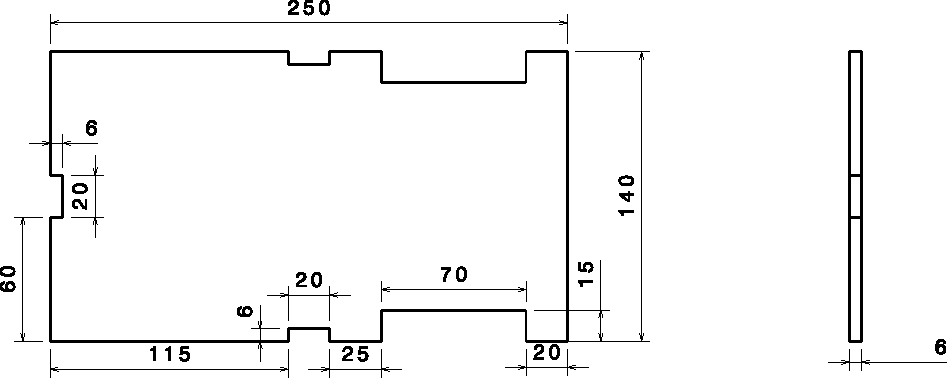
\includegraphics[scale=0.525,page=1]{../img/structure.pdf}
  \end{center}

  \legend{Fonte: Elaborado pelos autores.}
\end{figure}

\begin{figure}[htb]
  \caption{\label{fig:structure-side} Visão lateral do robô}

  \begin{center}
    \includegraphics[scale=0.525,page=2]{../img/structure.pdf}
  \end{center}

  \legend{Fonte: Elaborado pelos autores.}
\end{figure}

\begin{figure}[htb]
  \caption{\label{fig:structure-back} Visão traseira do robô}

  \begin{center}
    \includegraphics[scale=0.525,page=3]{../img/structure.pdf}
  \end{center}

  \legend{Fonte: Elaborado pelos autores.}
\end{figure}

\begin{figure}[htb]
  \caption{\label{fig:structure-front} Visão frontal do robô}

  \begin{center}
    \includegraphics[scale=0.525,page=4]{../img/structure.pdf}
  \end{center}

  \legend{Fonte: Elaborado pelos autores.}
\end{figure}

\begin{figure}[htb]
  \caption{\label{fig:structure-up} Visão superior do robô}

  \begin{center}
    \includegraphics[scale=0.525,page=5]{../img/structure.pdf}
  \end{center}

  \legend{Fonte: Elaborado pelos autores.}
\end{figure}

\begin{figure}[htb]
  \caption{\label{fig:structure-iso} Visão isométrica do robô}

  \begin{center}
    \includegraphics[scale=0.525,page=6]{../img/structure.pdf}
  \end{center}

  \legend{Fonte: Elaborado pelos autores.}
\end{figure}

%
% Comando para pular todo o conteúdo a seguir para a próxima página, para
% evitar que a figura fique no final da próxima seção.
%
\newpage

\section{Descrição de software}

Para realizar uma descrição precisa do software, foram utilizados oito artefatos
com o objetivo de esclarecer a maneira como o software será produzido. Os
artefatos são os seguintes:

\begin{enumerate}
  \item
    um diagrama do processo de negócio do problema que a máquina se propõe a
    resolver;
  \item lista de casos de uso (backlog funcional);
  \item lista de requisitos funcionais e não-funcionais;
  \item diagrama de casos de uso;
  \item diagrama de classes;
  \item diagrama de arquitetura;
  \item diagrama de estados da máquina; e
  \item
    descrição dos testes dos componentes da máquina e dos testes funcionais que
    deveriam ser feitos para avaliar o funcionamento da máquina e identificar
    defeitos.
\end{enumerate}

\subsection{Diagrama de Estados da Máquina}

\begin{figure}
  \caption{\label{fig:states} Diagrama de estados da máquina}

  \begin{center}
    \includegraphics[scale=0.625]{../diagrams/states.pdf}
  \end{center}

  \legend{Fonte: Elaborado pelos autores.}
\end{figure}


\chapter{Cronograma do Projeto}

\begin{xltabular}{\columnwidth}{X|X|X|X|X|X}
  \caption{\label{tabela_cronograma_projeto}Cronograma por Atividade} \\

  \hline
  \textbf{Atividade} & \textbf{Início previsto} & \textbf{Início realizado} & \textbf{Fim previsto} & \textbf{Fim realizado} & \textbf{Responsável} \\
  \hline
  \endfirsthead
  \multicolumn{6}{c}
  {\tablename\ \thetable\ -- \textit{Continuação da tabela}} \\
  \hline
  \textbf{Atividade} & \textbf{Início previsto} & \textbf{Início realizado} & \textbf{Fim previsto} & \textbf{Fim realizado} & \textbf{Responsável} \\
  \endhead
  \multicolumn{6}{r}{\textit{Continua na próxima página}} \\
  \endfoot
  \multicolumn{6}{r}{\textit{Fim da tabela}} \\
  \multicolumn{6}{c}{Fonte: Elaborado pelos autores.} \\
  \endlastfoot

  %
  % Dados da tabela
  %
  Definição geral do produto & 08/04/2024 & 08/04/2024 & 15/04/2024 & 15/04/2024 & Todos \\
  \hline

  Nivelamento de expectativas & 08/04/2024 & 08/04/2024 & 15/04/2024 & 15/04/2024 & Todos \\
  \hline

  Resumo & 17/04/2024 & 17/04/2024 & 23/04/2024 & 23/04/2024 & Sarah Loriato \\
  \hline

  Revisão bibliográfica (introdução) & 17/04/2024 & 17/04/2024 & 23/04/2024 & 23/04/2024 & Guilherme Elizeu \\
  \hline

  Legislações (introdução) & 17/04/2024 & 17/04/2024 & 23/04/2024 & 23/04/2024 & João Ricardo \\
  \hline

  Indicadores de mercado (introdução) & 17/04/2024 & 17/04/2024 & 23/04/2024 & 23/04/2024 & Pedro Ambrosio \\
  \hline

  Justificativa & 17/04/2024 & 17/04/2024 & 23/04/2024 & 23/04/2024 & Ana Caroline \\
  \hline

  Termo de abertura (indicadores) & 17/04/2024 & 17/04/2024 & 23/04/2024 & 23/04/2024 & Caio Alexandre \\
  \hline

  Termo de abertura (objetivos) & 17/04/2024 & 17/04/2024 & 23/04/2024 & 23/04/2024 & Alexandre Beck \\
  \hline

  Termo de abertura (mercado-alvo) & 17/04/2024 & 17/04/2024 & 23/04/2024 & 23/04/2024 & Thales Germano \\
  \hline

  Termo de abertura (requisitos) & 17/04/2024 & 17/04/2024 & 23/04/2024 & 23/04/2024 & João Pedro \\
  \hline

  Projeto conceitual do produto & 17/04/2024 & 17/04/2024 & 23/04/2024 & 23/04/2024 & Henrique Galdino \\
  \hline

  Estrura analítica do projeto & 17/04/2024 & 17/04/2024 & 23/04/2024 & 23/04/2024 & Luis Felipe \\
  \hline

  Revisão e complementação & 23/04/2024 & 23/04/2024 & 05/05/2024 & 05/05/2024 & Sarah Loriato e Caio Alexandre \\
  \hline

  Montagem do diagrama de blocos e esquemático do hardware & 08/05/2024 & 08/05/2024 & 13/05/2024 & 13/05/2024 & Sarah Loriato e Rafael Silva \\
  \hline

  Montagem do CAD & 15/05/2024 & 15/05/2024 & 20/05/2024 & 20/05/2024 & Guilherme Elizeu, Maria Eliza e Ana Caroline \\
  \hline

  Montagem do diagrama (BPMN) & 13/05/2024 & 13/05/2024 & 27/05/2024 & 27/05/2024 & Equipe de software \\
  \hline

  Montagem do diagrama de casos de uso & 13/05/2024 & 13/05/2024 & 27/05/2024 & 27/05/2024 & Equipe de software \\
  \hline

  Montagem do diagrama de classes & 13/05/2024 & 13/05/2024 & 27/05/2024 & 27/05/2024 & Equipe de software \\
  \hline

  Montagem do diagrama de arquitetura (C4) & 13/05/2024 & 13/05/2024 & 27/05/2024 & 27/05/2024 & Equipe de software \\
  \hline

  Montagem do diagrama de estados de máquina & 13/05/2024 & 13/05/2024 & 27/05/2024 & 27/05/2024 & Equipe de software \\
  \hline

  Definição e atribuição de responsabilidades e tarefas (software) & 27/05/2024 & 27/05/2024 & 27/05/2024 & 27/05/2024 & Equipe de software \\
  \hline

  Início da escrita de algoritmos & 27/05/2024 & 27/05/2024 & 08/06/2024 & --- & Equipe de software \\
  \hline

  Levantamento de materiais necessários para a montagem do seguidor de linha & 13/05/2024 & 13/05/2024 & 22/06/2024 & 22/05/2024 & Equipe de hardware e estruturas \\
  \hline

  Compra dos materiais & 14/05/2024 & 14/05/2024 & 25/06/2024 & 24/05/2024 & Sarah Loriato e Maria Eliza \\
  \hline

  Impressão 3D da estrutura & 23/05/2024 & 23/05/2024 & 25/06/2024 & 27/05/2024 & Sarah Loriato e Maria Eliza \\
  \hline

  Teste de integração dos componentes eletrônicos & 27/05/2024 & 27/05/2024 & 27/05/2024 & 27/05/2024 & Sarah Loriato e Rafael Silva \\
  \hline

  Corte dos materiais & 25/05/2024 & 24/05/2024 & 27/05/2024 & 28/05/2024 & Guilherme Elizeu, Ana Caroline e Maria Eliza \\
  \hline

  Pesquisa das propriedades dos componentes eletrônicos para análise energética & 15/05/2024 & 15/05/2024 & 20/05/2024 & 20/05/2024 & Pedro Ambrosio \\
  \hline

  Montagem parcial de diferentes blocos eletrônicos para testes direcionados de funcionamento & 28/05/2024 & 28/05/2024 & 29/05/2024 & 30/05/2024 & Sarah Loriato e Rafael Silva \\
  \hline

  Montagem total dos componentes eletrônicos (com todos os componentes e funcionalidades) & 30/05/2024 & --- & 02/06/2024 & --- & Sarah Loriato e Rafael Silva \\
  \hline

  Experimento com peso em hardware & 28/05/2024 & 28/04/2024 & 02/05/2024 & 02/05/2024 & Sarah Loriato e Rafael Silva \\
  \hline

  Montagem estrutural do seguidor de linha com as peças cortadas e impressão 3D & 29/05/2024 & 29/05/2024 & 05/06/2024 & --- & Guilherme Elizeu, Ana Caroline e Maria Eliza \\
  \hline

  Fixação do circuito eletrônico na estrutura do seguidor de linha & 05/06/2024 & --- & 05/06/2024 & --- & Equipe de hardware e estruturas \\
  \hline

  Teste de integração entre hardware e software & 10/06/2024 & --- & 12/06/2024 & --- & Equipe de hardware e software \\
  \hline

  Testes gerais & 12/06/2024 & --- & 21/06/2024 & --- & Todos \\
  \hline

  Análise de dados e ajustes finais & 22/06/2024 & --- & 26/06/2024 & --- & Todos \\
  \hline
\end{xltabular}


%
% Elementos pós-textuais
%
\postextual

%
% Referências bibliográficas
%
\bibliography{refs}

\end{document}
